% An implementable description of the improved process.
% (feel free to reference to little changed parts explained earlier)
% Changes with respect to model 1 Explain the changes you made
% and motivate on which performance criteria the model improves or
% worsens.
% Workflow patterns Highlight and motivate changes in workflow
% patterns. Feel free to refer to earlier parts in the report.
% Soundness Argue that the control flow of the process is sound.

\subsection{Description}
In this section we describe how we altered the process from Section~\ref{sec:model1} so that is comprehends to the new additional requirements, which are stated in \autoref{app:appendix_additional}.
We also made some improvements and these are also described in this section.
A complete overview of the second bizagi model van be found in \autoref{app:appendix_model2}.

The first change we made was in the first part right after the task \emph{fill out and send back forms}.
Now before we go to \emph{Check if forms are complete} we do an automatic check to see if the forms contain a valid IBAN.
If not we consider the forms as incomplete and the flow continues to \emph{Add explanation missing items}.
If it was correct the process continues to the task \emph{Check if forms are complete}. Since this check is done automatically, we do not need any employees for this.

The second change regards the payment via the bank. Before we had a task \emph{Payment via bank Student} and we assumed that this payment would always succeed.
Now we do not do that anymore. After this first payment task there is another task, \emph{Offer Payment to External Service}.
This service determines whether the payment succeeds, is delayed, fails or is invalid.
This decision is made by a random distribution which will be explained later.
The way the flow continues depends on the result of this task.

If the result is successful than the flow continues to the task \emph{Pick up Laptop}.
If the payment fails than the student has top pay for the laptop in cash when he comes to pick it up.
This means that the flow continues to the task \emph{Pay Laptop in Cash}.
If the payment is delayed then the flow returns to the task \emph{Offer Payment to External Service}, where it is tried again to do a payment.
The random distribution is chosen in such a way that it is not possible that one IBAN results in an infinite loop of delayed payments and therefore a deadlock in the process.
The last option was that the payment was invalid, this would be the case when the amount to be payed was negative but we do not allow these amounts in our model and therefore this option will never occur.

After the first simulation we noticed that almost everytime before the laptop arrives, the registration was already completed.
This was due to the fact that waiting fora laptop took much more time than completing the registration.
This also resulted in a  high resource utilization for the NSC employee since the employee was "busy waiting" in the \emph{Wait for notebook to arrive} task.
Therefore we splitted this task into two tasks. One is the original \emph{Wait for notebook to arrive}, but now without using resources, and the \emph{Notebook} arrive task.
This task is done by the NSC employee. This resolved the "busy waiting" problem.

We resolved the problem with the registration by adding the restraint that if a student wants to pay via the bank, a registration can only be completed when the notebook has arrived.
This means the task \emph{Register Student} can be executed only when the notebook has arrived.
If a student wants to pay in cash (most of the times this is the situation when a request is to late) the task \emph{Register Student} does not have to wait for the notebook to arrive.
We choose for this because in this case it does not matter that the student cannot pay via the bank anymore after the registration is completed, since he wants to pay in cash.
Another reason we chose for this is that we can imagine that,
when a request is to late (so the academic year is already started) you want to finish the registration as soon as possible, such that the student can participate in the courses.
The laptop is not immediately necessary to do this, but a complete registration is.

\begin{figure}[H]
	\centering
	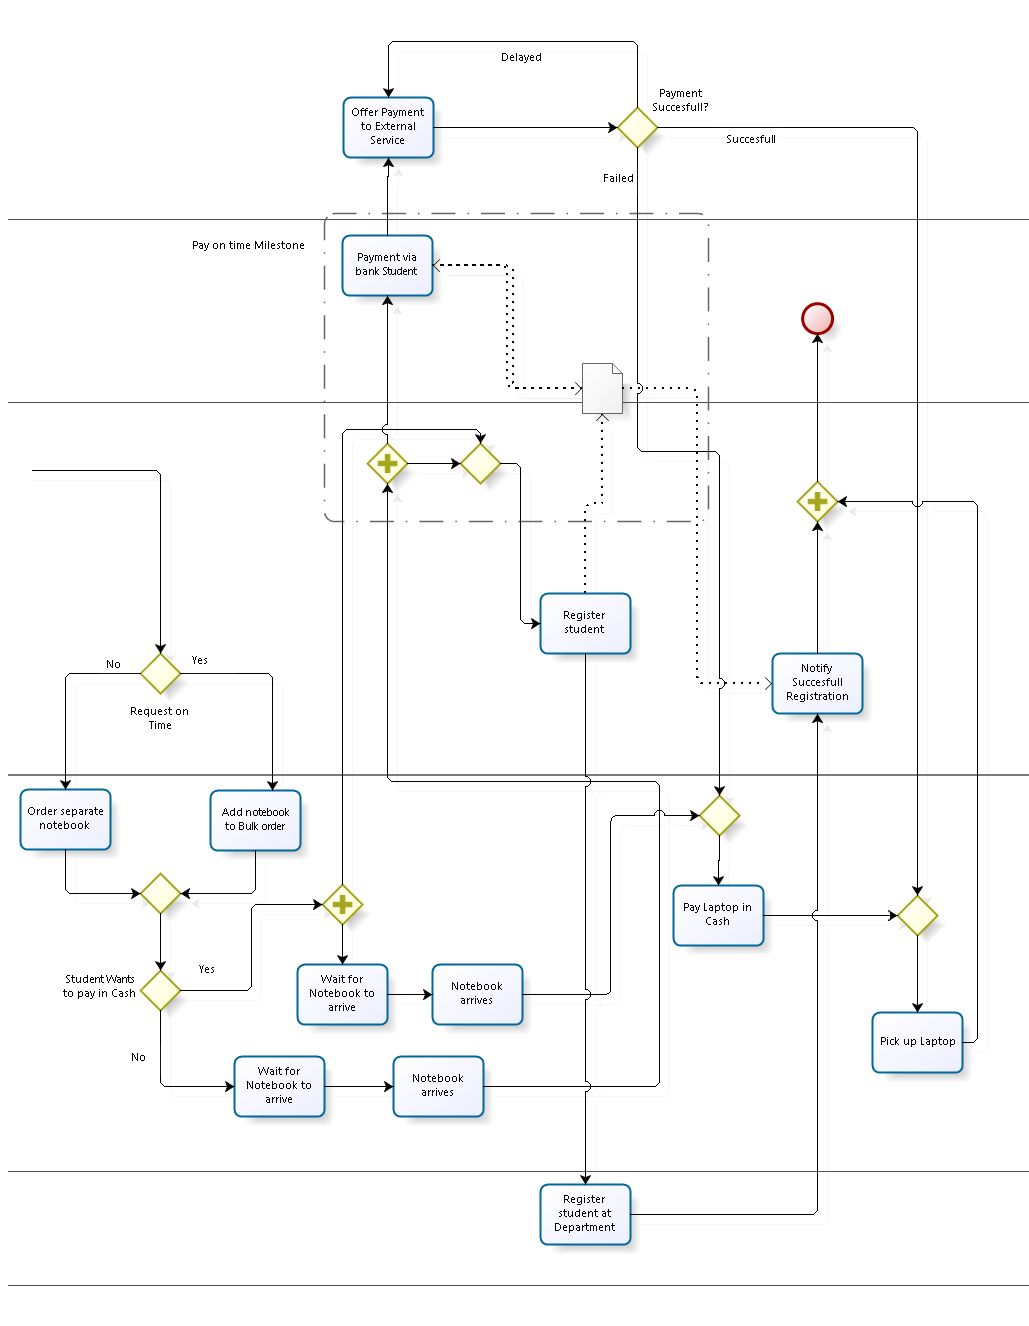
\includegraphics[scale=0.5]{model2-part1}
	\caption{The changed part of the second model in Bizagi}
	\label{fig:model2-part1}
\end{figure}

\subsection{Workflow patterns}

The workflow patterns in version 2 of the model are the same as those described in Section~\ref{sec:model1:patterns}.

\subsection{Soundness}

For the second model, we just used ProM to show soundness.

\subsubsection{ProM}

We used ProM to check the soundness of our model.
The resulting net can be seen in Appendix~\ref{app:prom}.

The Woflan analyzer gave the results we expected: aside from the fact that we have three ending places, the net is valid.
